% This work is licensed under the Creative Commons
% Attribution-NonCommercial-ShareAlike 4.0 International License. To view a copy
% of this license, visit http://creativecommons.org/licenses/by-nc-sa/4.0/ or
% send a letter to Creative Commons, PO Box 1866, Mountain View, CA 94042, USA.




\tikzset{every picture/.style={line width=0.75pt}} %set default line width to 0.75pt        

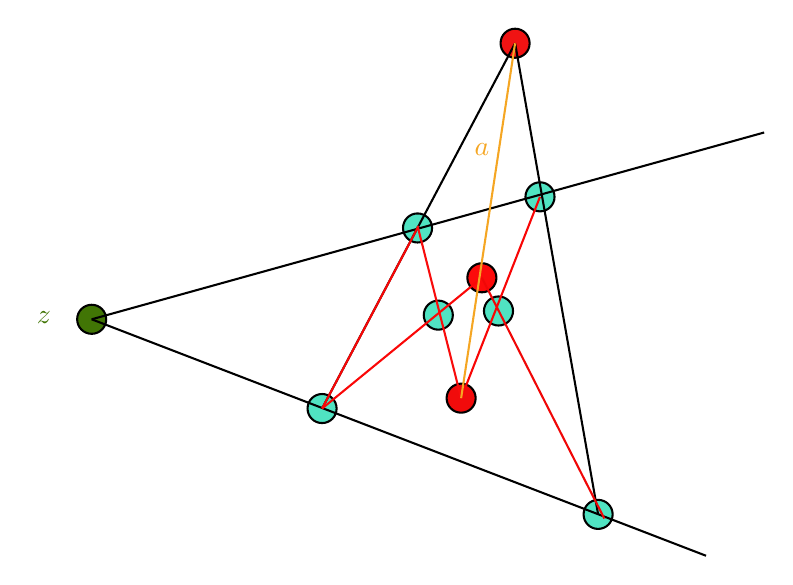
\begin{tikzpicture}[x=0.75pt,y=0.75pt,yscale=-1,xscale=1]
%uncomment if require: \path (0,300); %set diagram left start at 0, and has height of 300

%Shape: Circle [id:dp08312604554148328] 
\draw  [fill={rgb, 255:red, 80; green, 227; blue, 194 }  ,fill opacity=1 ] (192,142) .. controls (192,138.13) and (195.13,135) .. (199,135) .. controls (202.87,135) and (206,138.13) .. (206,142) .. controls (206,145.87) and (202.87,149) .. (199,149) .. controls (195.13,149) and (192,145.87) .. (192,142) -- cycle ;
%Shape: Circle [id:dp5479371678347926] 
\draw  [fill={rgb, 255:red, 80; green, 227; blue, 194 }  ,fill opacity=1 ] (182,100) .. controls (182,96.13) and (185.13,93) .. (189,93) .. controls (192.87,93) and (196,96.13) .. (196,100) .. controls (196,103.87) and (192.87,107) .. (189,107) .. controls (185.13,107) and (182,103.87) .. (182,100) -- cycle ;
%Shape: Circle [id:dp9035059763139627] 
\draw  [fill={rgb, 255:red, 241; green, 11; blue, 11 }  ,fill opacity=1 ] (203,182) .. controls (203,178.13) and (206.13,175) .. (210,175) .. controls (213.87,175) and (217,178.13) .. (217,182) .. controls (217,185.87) and (213.87,189) .. (210,189) .. controls (206.13,189) and (203,185.87) .. (203,182) -- cycle ;
%Shape: Circle [id:dp13405737177609034] 
\draw  [fill={rgb, 255:red, 65; green, 117; blue, 5 }  ,fill opacity=1 ] (25,144) .. controls (25,140.13) and (28.13,137) .. (32,137) .. controls (35.87,137) and (39,140.13) .. (39,144) .. controls (39,147.87) and (35.87,151) .. (32,151) .. controls (28.13,151) and (25,147.87) .. (25,144) -- cycle ;
%Shape: Circle [id:dp820938089239013] 
\draw  [fill={rgb, 255:red, 240; green, 19; blue, 19 }  ,fill opacity=1 ] (229,11) .. controls (229,7.13) and (232.13,4) .. (236,4) .. controls (239.87,4) and (243,7.13) .. (243,11) .. controls (243,14.87) and (239.87,18) .. (236,18) .. controls (232.13,18) and (229,14.87) .. (229,11) -- cycle ;
%Shape: Circle [id:dp9814130832419268] 
\draw  [fill={rgb, 255:red, 80; green, 227; blue, 194 }  ,fill opacity=1 ] (136,187) .. controls (136,183.13) and (139.13,180) .. (143,180) .. controls (146.87,180) and (150,183.13) .. (150,187) .. controls (150,190.87) and (146.87,194) .. (143,194) .. controls (139.13,194) and (136,190.87) .. (136,187) -- cycle ;
%Shape: Circle [id:dp7483452900473003] 
\draw  [fill={rgb, 255:red, 80; green, 227; blue, 194 }  ,fill opacity=1 ] (241,85) .. controls (241,81.13) and (244.13,78) .. (248,78) .. controls (251.87,78) and (255,81.13) .. (255,85) .. controls (255,88.87) and (251.87,92) .. (248,92) .. controls (244.13,92) and (241,88.87) .. (241,85) -- cycle ;
%Shape: Circle [id:dp47277380471474084] 
\draw  [fill={rgb, 255:red, 80; green, 227; blue, 194 }  ,fill opacity=1 ] (269,238) .. controls (269,234.13) and (272.13,231) .. (276,231) .. controls (279.87,231) and (283,234.13) .. (283,238) .. controls (283,241.87) and (279.87,245) .. (276,245) .. controls (272.13,245) and (269,241.87) .. (269,238) -- cycle ;
%Shape: Circle [id:dp9584244691590221] 
\draw  [fill={rgb, 255:red, 80; green, 227; blue, 194 }  ,fill opacity=1 ] (221,140) .. controls (221,136.13) and (224.13,133) .. (228,133) .. controls (231.87,133) and (235,136.13) .. (235,140) .. controls (235,143.87) and (231.87,147) .. (228,147) .. controls (224.13,147) and (221,143.87) .. (221,140) -- cycle ;
%Straight Lines [id:da8654056524389862] 
\draw    (32,144) -- (328,257.93) ;


%Straight Lines [id:da5764695965444305] 
\draw    (32,144) -- (356,54) ;


%Straight Lines [id:da5308065029099274] 
\draw    (236,11) -- (143,187) ;


%Straight Lines [id:da046230899122107094] 
\draw    (236,11) -- (276,238) ;


%Shape: Circle [id:dp5984512451328349] 
\draw  [fill={rgb, 255:red, 252; green, 11; blue, 11 }  ,fill opacity=1 ] (213,124) .. controls (213,120.13) and (216.13,117) .. (220,117) .. controls (223.87,117) and (227,120.13) .. (227,124) .. controls (227,127.87) and (223.87,131) .. (220,131) .. controls (216.13,131) and (213,127.87) .. (213,124) -- cycle ;
%Straight Lines [id:da11514776685343242] 
\draw [color={rgb, 255:red, 248; green, 12; blue, 12 }  ,draw opacity=1 ]   (189,99) -- (210,182) ;


%Straight Lines [id:da39941550536718873] 
\draw [color={rgb, 255:red, 250; green, 7; blue, 7 }  ,draw opacity=1 ]   (220,124) -- (143,187) ;


%Straight Lines [id:da1529104012025022] 
\draw [color={rgb, 255:red, 247; green, 6; blue, 6 }  ,draw opacity=1 ]   (189,100) -- (143,187) ;


%Straight Lines [id:da4295459927621441] 
\draw [color={rgb, 255:red, 240; green, 7; blue, 7 }  ,draw opacity=1 ]   (220,124) -- (279,240) ;


%Straight Lines [id:da36586521305300124] 
\draw [color={rgb, 255:red, 248; green, 5; blue, 5 }  ,draw opacity=1 ]   (248,85) -- (210,182) ;


%Straight Lines [id:da9039017754327724] 
\draw [color={rgb, 255:red, 245; green, 166; blue, 35 }  ,draw opacity=1 ]   (236,11) -- (210,182) ;



% Text Node
\draw (9,143) node [color={rgb, 255:red, 65; green, 117; blue, 5 }  ,opacity=1 ] [align=left] {$z$};
% Text Node
\draw (220,62) node [color={rgb, 255:red, 245; green, 166; blue, 35 }  ,opacity=1 ] [align=left] {$a$};


\end{tikzpicture}
